%&pdflatex

\documentclass[12pt]{report}

\usepackage{fancyhdr}
\usepackage{algorithm}
\usepackage{algpseudocode}
\usepackage{amsmath} % for implementation of the matrix environment
\usepackage{blindtext}
\usepackage{caption}
\usepackage{color}
\usepackage[pdftex]{graphicx} \graphicspath{{graphics/}}
\usepackage{epstopdf} \epstopdfsetup{update} % only regenerate pdf files when eps file is newer
\usepackage{float} % figure groups aka floats
\usepackage{forest} % for MFS elimination tree diagram
\usepackage[left=3.5cm, right=2.5cm]{geometry} % margins
\usepackage[shellescape,latex]{gmp} % metapost for UMLs
\usepackage[hidelinks]{hyperref} % ToC/LoA/LoF/LoT entries are links
\usepackage{mathptmx} % Times New Roman like font
\usepackage{pdfpages} % for inserting pdf as the initial pages
\usepackage{setspace} \onehalfspacing % 1.5 line spacing
\usepackage{subcaption}
\usepackage{xfrac} % nice slanted fractions
\usepackage{polski}
\usepackage[utf8]{inputenc}
\usepackage[T1]{fontenc}
\usepackage{indentfirst}

\captionsetup[figure]{labelfont={bf}, textfont={small}}
\captionsetup[subfigure]{labelfont={bf}, textfont={small}}

\newcommand{\bt}{\blindtext}
\newcommand{\eps}{\varepsilon}
%\newcommand{\rev}[1]{\textcolor{red}{#1}}
\newcommand{\rev}[1]{#1}
\newcommand{\T}[1]{\texttt{#1}}
\newcommand{\mychapter}[2]{
    \setcounter{chapter}{#1}
    \setcounter{section}{0}
    \chapter*{#2}
    \addcontentsline{toc}{chapter}{#2}
}

\algnewcommand\And{\,\textbf{and}\,}
\algnewcommand\Or{\,\textbf{or}\,}
\algnewcommand{\LineComment}[1]{\State \(\triangleright\) #1}


\begin{document}


\includepdf[pages={-,{}}]{initial-pages.pdf} % `-' for all pages, `{}' for an empty page

\tableofcontents


\chapter{State of the art}

\section{Planowanie ruchu na skrzyżowaniach}

Zależność wydajności od rozmiaru problemu

Szybkość zmian w środowisku uniemożliwia użycia algorytmu zajmującego dużo czasu

Rozważana klasa problemów

Porównanie metody deterministycznej i heurystycznej

Konieczność użycia metody heurystycznej z powodu dużej złożoności
\bt

\section{Planowanie ruchu przy użyciu świateł drogowych}

Opis dotychczasowych modeli ruchu przy użyciu świateł drogowych na podstawie artykułu [1]

Opis optymalizacji wprowadzonych do zarządzania sygnalizacją świetlną na podstawie artykułu [1]:
  - Synchronized Traffic Lights
  - Green Wave
  - Random Offset

Porównanie powyższych optymalizacji na podstawie artykułu [1]

Opis koordynacji ruchu przy użyciu algorytmu REAL TIME QUEUE LENGTH ESTIMATION: THE APTTC ALGORITHM na podstawie artykułu [7]:
  - Sterowanie adaptacyjne
  - Statystyczna optymalizacja
  - Estymacja na podstawia długości dynamicznej kolejki

Porównanie powyższego rozwiązania z synchroniczną zmianą świateł.

\section{Planowanie ruchu bez sygnalizacji świetlnej}

\bt

Znajdowanie ścieżki za pomocą algorytmu Dijkstr'y na podstawie artykułu [2]

Unikanie kolizji przy użyciu algorytmu Dijkstry' na podstawie artykułu [2]

Planowanie ruchu za pomocą zmodyfikowanego algorytmu A* na podstawie artykułu [3]

Planowanie ruchu za pomocą wielostanowego algorytmu A* oraz wielostanowego algorytmu Wavefront na podstawie artykułu [4]

Autonomiczne podejśćie - użycie Automated Guided Vehicels.

Planowanie ruchu oraz unikanie kolizji przy użyciu AGV na podstawie artykułu [8]

Omówienie przykładu z użyciem AGV na podstawie artykułu [8]

Omówienie agorytmów stosowanych do planowania drogi na podstawie artykułu [5]:
- Dijkstra's Algorithm
- Priority Queues
- Bidirectional Search
- A*

\section{State of the art}

\subsection{Technology 1}

A lot of bibliography citations here...

\bt

\subsection{Technology 2}

\bt

\section{Main thesis of this work}

The main thesis of this work may be expressed as follows:

\medskip

\textit{
	\bt
}


\mychapter{2}{Istniejące rozwiązania w zakresie planowania ruchu i koordynacji ruchu na skrzyżowaniach} \label{chap:state-of-the-art}

\section{Planowanie ruchu na skrzyżowaniach}

\textbf{Cel - lista wymagań i cech mojego rozwiązania - tego nie będzie w treści}
\newline
- Zastosowanie algorytmu A* do zaplanowania ruchu na skrzyżowaniach
\newline
- Brak świateł powinno przyspieszyć ruch na szkyżowaniach - auta nie czekają na świetle pomarańczowym
\newline
- Rozwiązanie uwzględnia unikanie kolizji
\newline
- A* powinien szybciej zaplanować drogę niż np. Dijkstra
\newline
- W rozwiązaniu zapewnione jest bezpieczeństwo - nie dochodzi do kolizji
\newline
- Rozwiązanie koordynuje ruch globalnie
\newline
\newline
\newline
\newline
\indent
  Planowanie ruchu zawsze wiąże się z rozmiarem problemu. Dla koordynacji ruchu na skrzyżowaniach o rozmiarze problemu stanowi rozmiar dróg, ich liczba oraz liczba przecięć między nimi, a także parametry i liczba pojazdów. Z planowaniem ruchu wiąże się trudność jaką jest szybkość zmian w środowisku. W przypadku nie zastosowania się pojazdu do planu, algorytm musi natychmiast wyliczyć poprawiony plan. System planujący ruch drogowy, powinien być więc systemem czasu rzeczywistego. Cechą takich systemów, jest równoległość w czasie zmian w środowisku oraz prowadzonych przez system obliczeń opierających się o stan środowiska. Algorytmy heurystyczne są najczęściej stosowane w wielokrotnie zmieniających się środowiskach.
\newline
\indent
Popularnym modelem reprezentującym sieci dróg jest graf. Wierzchołki grafu to skrzyżowania dróg. Krawędzie natomiast, reprezentują odległości między skrzyżowaniami za pomocą wag. Często stosowanym algorytmem do znajdowania najkrótszej ścieżki w grafie, jest algorytm Dijkstry \cite{shaikh2013agv}, \cite{ando2003autonomous}, \cite{huang2013improved}, \cite{gazis1997optimal}, \cite{broxmeyer1994vehicle}, \cite{kanoh2007dynamic}. O rzędzie złożoności algorytmu decyduje implementacja kolejki. W przypadku implementacji kolejki poprzez kopiec, złożoność algorytmu to:
\newline
\newline
\begin{math}
O(E + V\log V)
\end{math}
\newline
\newline
gdzie \begin{math}E\end{math} to liczba krawędzi grafu, a \begin{math}V\end{math} liczba wierzchołków grafu.
\indent
\newline
\newline
\indent
  Jednym z algorytmów heurystycznych, stosowanych do szukania najkrótszej ścieżki, jest Algorytm A* \cite{munteanmobile}, \cite{oleiwi2014modified}, \cite{wojnicki2015robust}, \cite{elhalawany2013modified}, \cite{dechter1985generalized}. Złożoność czasowa algorytmu, jest zależna od zastosowanej funkcji heurystyki. Jeśli funkcja heurystyki spełnia następujący warunek:
\newline
\newline
\begin{math}
|h(x)-h^{*}(x)|=O(\log h^{*}(x))
\end{math}
\newline
\newline
gdzie \begin{math}h^{*}\end{math} jest optymalną heurystyką - liczba przeszukanych węzłów rośnie wielomianowo w stosunku do długości rozwiązania.
\newline
\indent
W artykule \cite{wojnicki2015robust} autorzy przedstawili algorytm A*, w celu planowania wielowymiarowego. W celu przybliżenia złożoności jako przykładowe środowisko podana została dwuwymiarowa, dyskretna przestrzeń kwadratowa o boku 7. Pojazdy mogą zajmować wówczas 49 pozycji oznaczonych współrzędnymi \begin{math}(x, y)\end{math}. Dla jednego pojazdu, możliwość zajmowanych pozycji wynosi \begin{math}(7 * 7) = 49 \end{math}. Dla dwóch pojazdów jest to już \begin{math}(7 * 7) * (7 * 7 - 1) = 2352 \end{math}. Aktualny stan jest wówczas opisywany jako \begin{math}(x1, y1, x2, y2)\end{math}. Złożoność rośnie wraz z przetrzymywaniem kolejnych informacji na temat pojazdów, czyli na przykład prędkości czy przyspieszenia.
\newline
\indent
Autorzy artykułu \cite{leena2014survey} zwrócili uwagę na podział planowania na globalne i lokalne. W podejściu globalnym, dla algorytmu musi być znane całe środowisko, co wiąże się z dużym obciążeniem pamięciowym - algorytm przechowuje informacje na temat stanów wszystkich pojazdów na skrzyżowaniach. W podejśyiu lokalnym, środowisko dla pojedynczego pojazdu nie jest znane, algorytm poznaje je w czasie rzeczywistym. W przedstawionym rozwiązaniu zastosowane jest podejście globalne.

\section{Planowanie ruchu przy użyciu świateł drogowych}

\indent
Najczęściej stosowanym systemem do koordynacji ruchu na skrzyżowaniach są światła drogowe. Powodują one opóźnienia wiążące się z oczekiwaniem przy świetle pomarańczowym, które jednocześnie zapewnia bezpieczeństwo. Powstało wiele optymalizacji świateł drogowych w celu przyspieszenia ruchu na skrzyżowaniach.
\newline
\indent
W artykule \cite{brockfeld2001optimizing} autorzy opisują następujące optymalizacje sygnalizacji świetlnej: \textit{Synchronized Traffic Lights, Green Wave, Random Offset}. Synchroniczne światła drogowe oparte są o obliczane cykle oraz o klastry samochodów poruszających się po skrzyżowaniach. Klaster samochodów rusza, gdy pojawi się światło zielone. Pierwszy samochód rusza z największym przyspieszeniem, aż dojedzie do następnego skrzyżowania. Wówczas natychmiast włącza się światło czerwone i reszta samochodów w klastrze dojeżdża do skrzyżowania. Cykle są obliczane w sposób, aby opóźnienia były najmniejsze. Zgodnie ze zdaniem autorów, jedną z wad jest fakt, że rozwiązanie działa najlepiej dla cykli, które nie występują na rzeczywistych skrzyżowaniach. W celu usprawnienia, autorzy zaproponowali strategię zielonej fali. Głównym celem tego podejścia jest to, aby duże klastry samochodów były w ruchu. W artykule, strategia zielonej fali daje lepsze efekty niż strategia synchronicznych świateł. Ostatnią przedstawioną strategią jest losowa zmiana świateł przed skrzyżowaniami. W przeciwieństwie do poprzednich strategii - światła na skrzyżowaniach nie przełączają się jednocześnie. Użycie tej strategii powoduje powstawanie dużych klastrów samochodów na niektórych drogach i szybki przepływ na innych. Globalnie, strategia zielonej falii przynosiła najlepsze efekty. Przedstawione rozwiązania, muszą jednak stosować światło pomarańczowe w celu utrzymania bezpieczeństwa, co powoduje opóźnienia na każdym skrzyżowaniu.
\newline
\indent
Autorzy artykułu \cite{athmaraman2005adaptive} opisują koordynację ruchu przy użyciu algorytmu 'REAL TIME QUEUE LENGTH ESTIMATION: THE APTTC ALGORITHM'. Koordynacja ta działa przy użyciu tablicy sensorów fotoelektrycznych rozmieszczonych na drogach przy skrzyżowaniach. Algorytm w zależności od danych i estymacji kolejek, odpowiednio steruje sygnalizacją świetlną w celu uniknięcia opóźnień. Algorytm został uruchomiony w mieście Chennai w Indiach, gdzie wyestymowane zostały długości kolejek aut na drogach poprzez zamontowane sensory na każdy dzień tygodnia. Rozwiązanie jest jednak zaprojektowane do działania na jednym skrzyżowaniu oraz nie eliminuje opóźnień spowodowanych światłem pomarańczowym. Co więcej, w rozwiązaniu konieczne jest montowanie sensorów na drogach.
\newline
\indent
W artykule \cite{de1998optimal} opisane zostało kierowanie ruchem drogowym na jednym skrzyżowaniu poprzez optymalizację kolejek. W rozwiązaniu brane pod uwage są takie dane, jak średni czas oczekiwania, średnia długość kolejki i najgorszy czas oczekiwania. Istnieje także możliwość przekazania parametrów odpowiadających za maksymalny czas trwania światła czerwonego oraz zielonego. Wynikiem rozwiązania jest schemat zmiany świateł, który liczony jest za pomocą funkcji obiektowych na podstawie długości kolejek. W rozwiązaniu pominięty został element bezpieczeństwa jakim jest światło pomarańczowe. Rozwiązanie zostało pokazane także na jednym skrzyżowaniu, a nie na całej sieci skrzyżowań.
\newline
\indent
  Autorzy artykulu \cite{lammer2008self} przedstawili system kontroli świateł i przepływu pojazdów na sieciach drogowych. Rozwiązanie stosowane jest dla całych sieci skrzyżowań. Autorzy opierają się o krótkie prognozu ruchu i na ich podstawie liczą długość trwania światła zielonego. Klasyczne rozwiązania działają na wcześniej obliczonych danych oraz działają we wcześniej określonych miejscach największego ruchu. Takie rozwiązania powodują, że zielona fala trwa dużej niż powinna. W rozwiązaniu zastosowana jest także strategia stabilizacji, która zapewnia fakt, iż długość kolejek nie będzie zbyt długa. Zapewnione jest to przez odpowiednią długość trwania światła zielonego. W rozwiązaniu, na każdym ze skrzyżowań, samochody będą tracic czas na świetle pomarańczowym, które w rozwiązaniu jest konieczne, aby było ono bezpieczne. Ruch jest także optymalizowany dla sytuacji "średnich", które tak na prawdę nigdy nie występują. Wynikiem tego zjawiska jest fakt, że optymalizacja nigdy nie jest stosowana dla prawdziwej, aktualnej sytuacji.
\newline
\indent
W artykule \cite{ferreira2010self} przedstawiony został system zarządzania światłami za pomocą komunikacji pojazdów między sobą. Działanie systemu opiera się o sensory zamontowane przy skrzyżowaniach oraz urządzenia DSRC zamontowane w każdym z aut. Pojazdy komunikują się ze sobą za pomocą sieci bezprzewodowej, posiadają te same wersje map oraz posiadają GPS z dokładnością do pasa na którym się znajdują. W zależności od zebranych danych system odpowiednio przełącza światła w celu uniknięcia opóźnień. Przedstawione rozwiązanie jest kosztowne oraz pominięta jest kwestia bezpieczeństwa, która w innych rozwiązaniach zapewniona jest poprzez oczekiwanie na świetle pomarańczowym.
    
\section{Planowanie ruchu bez sygnalizacji świetlnej}

W celu uniknięcia użycia świateł drogowych, istnieją także rozwiązania z wykorzystaniem algorytmów znajdujących najkrótszą ścieżkę. W artykule \cite{shaikh2013agv} autorzy wykorzystali algorytm Dijkstry do zarządzania ruchem przy użyciu automatycznie prowadzonych pojazdów. Autorzy przedstawili zarządzanie ruchem pojazdów w magazynie chcąc ograniczyć czas transportu. Algorytm Dijkstry wskazuje najkrótszą ścieżkę od jednego pojazdu do następnego. W przypadku, gdy na ścieżce znajdzie się przeszkoda - algorytm wylicza ścieżkę od nowa. Zastosowanie algorytmu Dijkstry do koordynacji ruchu na skrzyżowaniach jest zbyt złożone. Ponadto, unikanie kolizji jest wykonane poprzez ponowne wyliczanie najkrótszej ścieżki, zamiast unikania ich na bieżąco.
\newline
\indent
Autorzy artykułu \cite{huang2013improved} przedstawiają ulepszoną wersję algorytmu Dijkstry w celu znalezienia najkrótszej ścieżki. Do algorytmu Dijkstry wprowadzona została funkcja, dzięki której ignorowane są nieistotne wierzchołki w grafie. Dzięki tej modyfikacji algorytm jest ~43\%-76\% szybszy. Rozwiązanie jest nadal zbyt złożone, by zastosować je do koordynacji ruchu na skrzyżowaniach. W rozwiązaniu nie ma także uwzględnionego unikania kolizji.
\newline
\indent
W artykule \cite{ando2003autonomous} przedstawione zostało planowanie ruchu przy użyciu automatycznie prowadzonych pojazdów wraz z unikaniem kolizji. W rozwiązaniu, każdy robot indywidualnie liczy najkrótszą dla siebie ścieżkę. Następnie, dane tras są wymieniane pomiędzy robotami, w celu ustalenia finalnego rozwiązania. Szukanie ścieżki jest wykonywane przy użyciu algorytmu Dijkstry. W celu unikania kolizji dla każdego pojazdu, liczona jest funkcja kary. Waga kary jest zwiększana tak długo, aż zostanie znaleziona bezkolizyjna ścieżka. Złożoność rozwiązania jest zbyt duża by zastosować je dla skrzyżowań. Wymienianie danych pomiędzy pojazdami oraz podany w rozwiązaniu sposób rozwiązywania kolizji, nie znajduje zastosowania w koorydynacji ruch na skrzyżowaniach.
\newline
\indent
W patencie \cite{gazis1997optimal} autorzy przedstawili centralnie zaplanowany, generalny system przydzielający trasy, w celu utrzymania optymalnego ruchu. System zawiera dużą ilość komputerów zamontowanych w pojazdach w celu komunikacji między nimi, poprzez sieć bezprzewodową. Do znajdowania najkrótszej ścieżki, autorzy wykorzystali algorytm Dijkstry. Ścieżki liczone są przy użyciu danych dostarczanych przez komputery zamontowane w pojazdach. Celem patentu jest znalezienie drogi do celu w najkrótszym czasie poprzez omijanie zakorkowanych dróg. Nie jest to dokładne zaplanowanie poruszania się pojazdu wraz z unikaniem kolizji.
\newline
\indent
Autorzy patentu \cite{broxmeyer1994vehicle} opisali system do kontroli ruchu i unikania kolizji na autostradach. Pod uwagę wzięte zostały zmiany pasów, unikanie kolizji oraz kontrolowanie trasy pojazdu. Unikanie kolizji zostało zapewnione poprzez komunikacje przez transmitery radiowe oraz radioodbiorniki zamontowane w każdym z pojazdów. Rozwiązanie znajduje zastosowanie na autostradach. Unikanie kolizji ma miejsce na równoległych pasach. Tego podejścia nie da się zastosować jeżeli chodzi o koordynacje ruchu na skrzyżowaniach.
\newline
\indent
W artykule \cite{kanoh2007dynamic} przedstawiony został system dynamicznego planowania ruchu do nawigacji samochodów przy użyciu 'virus genetic algorithms'. Autorzy zaproponowali algorytm genetyczny, który jest bardziej wydajny od algorytmu A*, czy algorytmu Dijkstry. W rozwiązaniu zastosowana jest strategia infekcji wirusowej, dzięki czemu omijane są korki na drogach. Rozwiązanie jest zaprojektowane do wskazania najlepszej trasy, nie jest to dokładne zaplanowanie ruchu samochodów wraz z wymijaniem kolizji.

\section{Użycie algorytmu A* do planowania ruchu}

\indent
Algorytm A* jest często stosowany do szukania najkrótszej ścieżki oraz planowania ruchu. W artykule \cite{dechter1985generalized} omówiona została optymalność tego algorytmu oraz funkcja heurystyki. A* jest algorytmem heurystycznym, który znajduje najkrótszą ścieżkę w grafie ważonym z dowolnego podanego wierzchołka do wierzchołka celu. Wierzchołkiem celu jest wierzchołek spełniający zadane warunki wygranej. W artykule przedstawione zostały poprzednie próby udowodnienia optymalności algorytmu. Autorzy przeprowadzili także własny dowód na optymalność algorytmu A*. Dowód polega na fakcie, iż kiedy funkcja heurystyki nigdy nie przeszacowuje, wtedy algorytm A* jest optymalny. Dla grafu, algorytm A* od zadanego wierzchołka startowego tworzy ścieżkę, wybierając niezbadany sąsiedni wierzchołek. Wybiera go w sposób aby minimalizować funkcję:
\newline
\newline
\begin{math} f(x) = g(x) + h(x)\end{math}
\newline
\newline
gdzie:
\newline
\newline
\begin{math} g(x) \end{math} to suma wag krawędzi od wierzchołka startowego do wierzchołka x, a
\begin{math} h(x) \end{math} to przewidywana przez funkcję heurystyki suma wag z wierzchołka x do wierzchołka docelowego.
\newline
\indent
W artykule \cite{delling2009engineering} autorzy przeprowadzili porównanie algorytmów do planowania drogi. Na początku omówiony został algorytm Dijkstry, aby później pokazać algorytmy od niego szybsze. Następnie, autorzy przedstawiają kolejki priorytetowe jako implementację algorytmu Dijkstry, które są w stanie poprawić jego złożoność z \begin{math} O(n^2) \end{math} do \begin{math} O(nlogn) \end{math}. Używanie kolejek priorytetowych nie sprawdza się jednak na bardzo dużych zbiorach danych. Następną zaproponowaną modyfikacją algorytmu Dijkstry jest wyszukiwanie dwukierunkowe. Algorytm równolegle uruchamia algorytm Dijkstry, w stronę celu oraz w stronę startu. Kiedy wierzchołek jest odwiedzony z dwóch strony, ścieżka może być znaleziona. Kolejno opisany został Algorytm A* korzystający z funkcji heurystyki, opartej o odległość Euklidesową. Według autorów znajdywanie najkrótszej ścieżko jest niewiele przyspieszone. Mimo to czas wykonania algorytmu A* jest krótszy od czasu wykonania algorytmu Dijkstry.
\newline
\indent
Wykorzystanie modyfikacji algorytmu A* wraz z algorytmem Wavefront zostało przedstawione w artykule \cite{wojnicki2015robust}. Autorzy przedstawili wersję algorytmu A*, która operuje na stanach. Autorzy pokazali przykład na dwuwymiarowej, dyskretnej przestrzeni kwadratowej o boku 7. Stanem początkowym jest rozłożenie czterech obiektów na rogach zadanej przestrzeni. Stanem końcowym natomiast, jest znalezienie się tych czterech obiektów po przeciwnych stronach przekątnych. Algortym Wavefront został zastosowany w celu otrzymania planów wielowariantowych dla obiektów. Zastosowanie algorytmu A* operującego na stanach wraz z prędkościami pojazdów wnosi duże narzuty obliczeniowe. Przeprowadzenie koordynacji ruchu dla dużych sieci skrzyżowań używając algorytmu A* wraz z Wavefront jest zbyt złożone.
\newline
\indent
W artykule \cite{elhalawany2013modified} autorzy zaproponowali modyfikację algorytmu A*, która skupia się na bezpieczeństwie w problemie nawigacji robotów. Modyfikacja polega na wzięciu pod uwagę rozmiaru robota oraz unikanie ostrych skrętów jeżeli chodzi o bezpieczeństwo. Do algorytmu A* przekazywany jest stan początkowy oraz cel jaki robot ma osiągnąć. Rozwiązanie przedstawione jest dla pojedynczego pojazdu, który ma za zadanie znaleźć najprostszą i bezpieczną ścieżkę wraz z unikaniem statycznych kolizji. Tego podejścia nie da się zastosować dla wielu pojazdów poruszających się po sieci skrzyżowań.

\section{Modyfikacje A*}

\indent
Autorzy artykułu \cite{munteanmobile} opisali modyfikację algorytmu A* do planowania ruchu. Rozwiązanie zostało zaprezentowanie dla robotów mobilnych. Autorzy stwierdzają fakt, że algorytm A* dla dużych danych potrzebuje dużo pamięci żeby śledzić dane, które są związane z aktualnym wierzchołkiem. Wspomniana została także modyfikacja algorytmu A*, która polega na równoczesnym przeszukiwaniu grafu w dwóch kierunkach. Kolejną modyfikacją jest IDA*, która nie używa pamięci do przechowywania wcześniej odwiedzonych wierzchołków. Minusem tej modyfikacji jest fakt, iż IDA* odwiedza niektóre wierzchołki wiele razy. Na końcu, autorzy zaproponowali swoją modyfikację - Fast A*. W modyfikacje zamiast list, użyte zostały drzewa binarne w celu przechowywania danych. W wyniku pracy zmodyfikowany algorytm Fast A* dawał lepsze wyniki od wersji klasycznej. Przedstawione modyfikacje są oparte o działanie na grafie, polegające na znalezieniu najkrótszej ścieżki z punktu startowego do punktu końcowego. Modyfikacje nie są wstanie wskazać najkrótszej ścieżki dla stanu początkowego i końcowego, którym może być na przykład położenie wszystkich samochodów na skrzyżowaniach.
\newline
\indent
W artykule \cite{oleiwi2014modified} autorzy zaproponowali genetyczny algorytm oparty na zmodyfikowanym algorytmie A* w celu optymalizacji znajdowania ścieżek dla wielu obiektów. Modyfikacja algorytmu A* polega na znalezieniu ścieżki suboptymalnej poprzez dodanie do algorytmu funkcji prawdopodobieństwa. Uniknięto więc szukania najkrótszej ścieżki, aby zwiększyć optymalność algorytmu. To rozwiązanie następnie jest przekazywane do algorytmu genetycznego. W rozwiązaniu uwzględnione zostało także unikanie kolizji. Autorzy opisali podejście optymalizacji szukania najkrótszej ścieżki dla pojedynczego pojazdu z unikaniem kolizji ze statycznymi elementami. Tego rozwiązania nie da się zastosować w sieci skrzyżowań, na której znajduje się wiele aut.
\newline
\indent
W celu planowania ruchu na skrzyżowaniach zostało przedstawione sporo rozwiązań. Większość z nich opiera się o stosowanie świateł. Powyżej zostały opisane optymalizacje świateł w celu przyspieszania ruchu drogowego. Rozwiązania te gwarantują bezpieczeństwo poprzez czekanie na świetle pomarańczowym, co powoduje kilkusekundowe straty na każdym skrzyżowaniu. Takich opóźnień nie ma stosując planowanie algorytmem. Przedstawione rozwiązania przy użyciu algorytmów planowania często nie brały pod uwagę unikania kolizji lub planowały jedynie ruch dla pojedynczego pojazdu. Tych podejść nie da się zastosować w celu zaplanowania ruchu na sieci skrzyżowań dla kilkunastu pojazdów.

\chapter{Teza} \label{chap:thesis}

\bt

\section{Podrozdział}

\bt

\section{Podrozdział}

\bt 

\section{Podrozdział}

\bt 

\mychapter{4}{4. Implementacja} \label{chap:implementation}

\section{Opis modelu danych do reprezentacji skrzyżowań}

W opracowanym rozwiązaniu drogi reprezentowane są w sposób dyskretny. Każda droga zaczyna się w pozycji 1 i rośnie wraz z jej rozmiarem. Droga jest opisywana przez:
\begin{itemize}
\item Unikatowy numer drogi
\item Rozmiar drogi
\item Informacja o przecięciach z innymi drogami
\item Kierunek w którym samochód się porusza na drodze (z północy na południe, czy z południa na północ lub z zachodu na wschód czy ze wschodu na zachód)
\end{itemize}
Samochody na drogach są opisane przez:
\begin{itemize}
\item Unikatowy numer samochodu
\item Unikatowy numer drogi, na której pojazd się znajduje
\item Numer pozycji na drodze, na której samochód się znajduje
\item Prędkość początkową
\item Numer pozycji docelowej na drodze - punkt za ostatnim skrzyżowaniem
\end{itemize}
Samochody poruszają się po drogach w krokach czasowych. Prędkość samochodu wyrażana jest w liczbie odcinków drogi na jeden krok czasowy.
\newline
\indent
W systemie można wybrać maksymalne przyspieszenia ujemne oraz dodatnie samochodów z następujących możliwości \{-2, -1, 0, 1, 2\}. Oznacza to, że w następnym stanie pojazd może przyspieszyć o 1 lub 2 odcinki drogi na jeden krok czasowy. Dla wartości 0 pojazd utrzymuje swoją prędkość. Dla wartości ujemnych pojazd zwalnia o 1 lub 2 odcinki drogi na jeden kroku czasowym. Ilość możliwych dla samochodu przyspieszeń znacznie wpływa na złożoność czasową algorytmu, z tego względu, że wraz ze wzrostem ilośći możliwych przyspieszeń rośnie ilość możliwość stanów sąsiednich dla samochodu, przez które algorytm musi przejść.        
\newline
\indent
Do modelu przekazać należy także maksymalną prędkość, którą wszystkie samochody mogą osiągnąć oraz parametr bezpieczeństwa, czyli liczba pozyji będąca dystansem trzymanym między pojazdami. W rozwiązaniu brane są pod uwage pomyłki pojazdów, które polegają na niezastosowaniu się do planu. Dzięki parametrowi bezpieczeństwa maleje prawdopodobieństwo kolizji, kiedy taka pomyłka będzie miała miejsce.

\section{Zmodyfikowany algorytm A*}

Zaprezentowany w tej pracy zmodyfikowany algorytm A* jest oparty na stanach, gdzie pojedyńczym stanem jest rozłożenie samochodów na drogach wraz z ich prędkościami. Algorytm zaczynając od zadanego stanu początkowego analizuje możliwe stany sąsiednie i wybiera najszybszą ścieżkę kierując się funkcją heurystyki. Ścieżka prowadzi do określonego celu. W przypadku opracowanego rozwiązania, celem jest przekroczenie przez wszystkie samochody ostatniego skrzyżowania na drogach, na których się znajdują.
\newline
\indent
Zrealizowany Algorytm A* jest generyczny. Do algorytmu przekazujemy klasę reprezentującą dowolny stan. Klasa musi implementować metodę 'neighbours', która zwraca stany sąsiednie dla danej instancji stanu. Do algorytmu przekazywana jest także funkcja heurystyki, zależna od danych danego stanu.
\newline
\indent
Modyfikacja róźni się od innych tym, że stany sąsiednie są liczone dynamicznie. Algorytm nie ma z góry podanego celu. Dla przykładu w przeszukiwaniu ścieżki w grafie celem jest podany wierzchołek końcowy. Algorytm przyjmuje funkcje wygranej, która określa warunki końca algorytmu. W przedstawionej pracy warunkiem końca jest przekroczenie przez wszystkie pojazdy skrzyżowań, a takich stanów jest wiele i nie są znane na początku działania.

\section{Stan w opracowanym rozwiązaniu dla algorytmu A*}

Stan w modyfikacji algorytmu A* przedstawionej w tej pracy opisuje stan wszystkich samochodów na skrzyżowaniach wraz z ich prędkościami. Zgodnie z wcześniej opisaną generycznością wierzchołek jest obiektem klasy, który implementuje metodę 'neighbours'. Metoda generuje wszystkie stany sąsiednie dla aktualnego stanu. Dla przykładu, dla ustawień przyspieszeń \{-2, -1, 0, 1, 2\}, dla każdego z aut na skrzyżowaniu generowane są stany z jego prędkością dodając wartości przyspieszeń. Pomijane są stany, w których prędkość samochodu byłaby ujemna. Przykładowo jest pojazd z prędkością 1 pozycji na krok czasowy znajdujący się na 1 pozycji na drodze numer 1. Dla pojazdu rozpatrywane są następujące stany:
\begin{enumerate}
\item Dodając przyspieszenie o wartości 0: 2 pozycja na drodze numer jeden z prędkością 1
\item Dodając przyspieszenie o wartości 1: 3 pozycja na drodze numer jeden z prędkością 2
\item Dodając przyspieszenie o wartości 2: 4 pozycja na drodze numer jeden z prędkością 3
\item Dodając przyspieszenie o wartości -1: 1 pozycja na drodze numer jeden z prędkością 0
\item Dodając przyspieszenie o wartości -2: Stan jest eliminowany, ponieważ prędkość byłaby ujemna
\end{enumerate}
Dodatkowo w przypadku ustawienia maksymalnej prędkości równej 2 pozycje na jeden krok czasowy - możliwość nr 3 także zostałaby wyeliminowana.
\newline
\newline
W metodzie usuwane są także stany powodujące kolizje, co będzie opisane w następnym rozdziale.

\section{Bezpieczeństwo ruchu i plany wielowariantowe}

W rozwiązaniu zaimplementowane zostało symulowanie pomyłek pojazdów. Pomyłka polega na niezastosowaniu się pojazdu do przekazanego mu planu. Bezpieczeństwo zapewnione jest przez parametr bezpieczeństwa. Parametrem bezpieczeństwa jest liczba odcinków drogi utrzymywana między pojazdami. Wartość parametru można przekazać do systemu.
\newline
\indent
Rozwiązanie zostało uruchamiane na jednym wątku procesora. W przypadku wykorzystania wielu wątków, metoda może wyliczyć plany dla pojazdów przewidując ich pomyłki. Dla przykładu, mając 4 pojazdy na skrzyżowaniu dwóch dróg załóżmy, że w każdym kroku czasowym jeden z nich, myli się z pewnym prawdopodobieństem o jeden odcinek drogi. Wyliczone wcześniej plany, z góry przewidując takie pomyłki - dostarczają nowy, poprawny plan. Takie rozwiązanie korzystając z nowych, poprawionych planów zmniejsza prawdopodobieństwo kolizji, w razie pomyłek pojazdów.

\section{Unikanie kolizji}

Koniecznym elementem w koordynacji ruchu na skrzyżowaniach wielu pojazdów jest unikanie kolizji. W opracowanym rozwiązaniu unikanie kolizji zostało podzielone na dwa etapy:
\begin{enumerate}
\item Unikanie kolizji aut poruszających się po tym samym pasie
\item Unikanie kolizji na skrzyżowaniach
\end{enumerate}
Implementacja unikania kolizji pojazdów na tym samym pasie polega na policzeniu obszarów dla samochodów znajdujących się na tym samym pasie, który będą one obejmowały w jednym kroku czasowym wraz z uwzględnieniem parametru bezpieczeństwa. Jeżeli obszary dwóch samochdów na jednym pasie pokrywają się - taki stan jest usuwany i wówczas metoda 'neighbours' nie zwróci go jako stanu sąsiedniego. Na rysunku \ref{collision-avoidance-lane} przedstawiony jest przykład unikania kolizji dla samochodów poruszających się jednym pasem. Przykład przedstawiony jest z parametrem bezpieczeństwa równym jeden. Samochody, mając przed sobą inny pojazd, czekają aż będzie dla nich miejsce. Stan pierwszy jest stanem startowym. Kolejno w stanie drugim, pojazd \textbf{D} rusza i zmienia swoją pozycję o jeden do przodu, ponieważ nie ma żadnego pojazdu przed nim. Reszta pojazdów stoi i czeka na miejsce. Następnie w stanie trzecim, pojazd \textbf{C} widząc, że ma miejsce porusza się o jedną pozycję do przodu. W stanie następnym na miejsce czeka jedynie samochód \textbf{A} - reszta zmienia pozycję. W kroku piątym i szóstym pojazdy mając miejsce, swobodnie opuszczają skrzyżowanie.
\begin{figure}[H]
    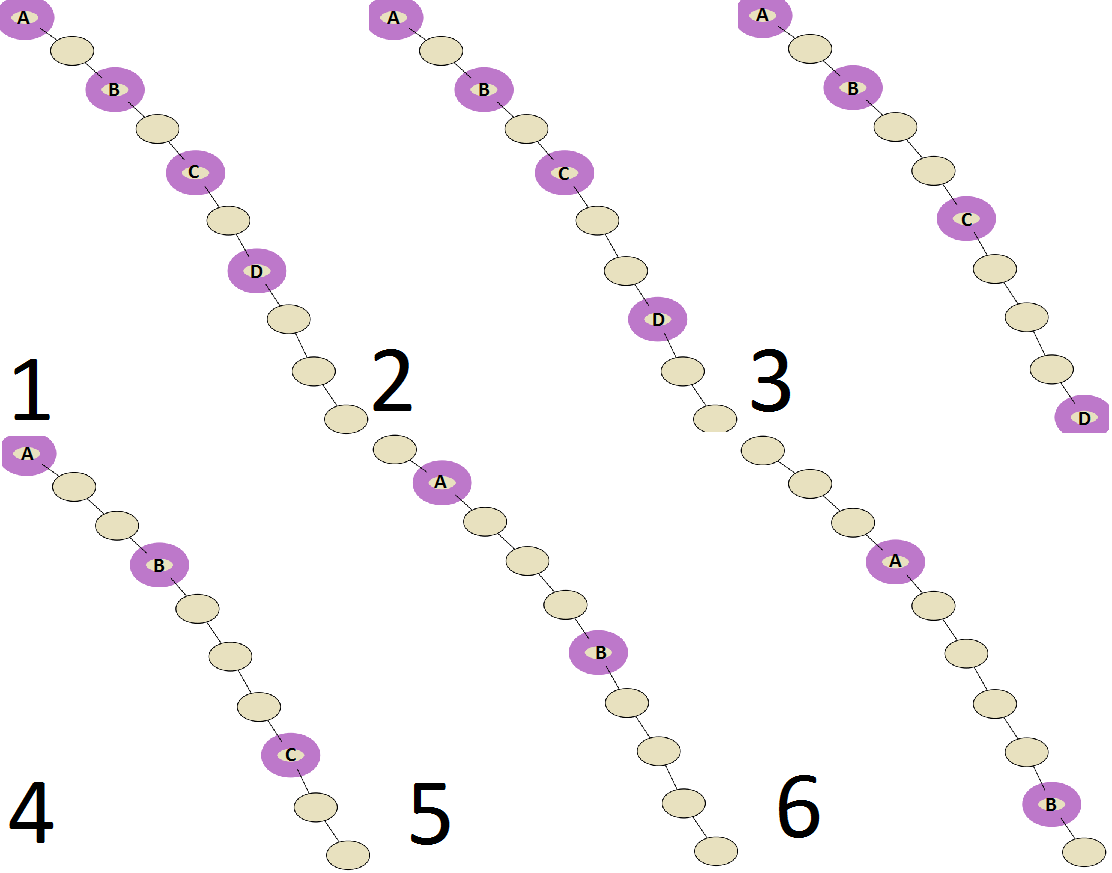
\includegraphics[width=1.0\textwidth]{collision-avoidance-lane.png}
  \caption{Unikanie kolizji na pasie}
  \label{collision-avoidance-lane}
\end{figure}
\newpage
Unikanie kolizji na skrzyżowaniach polega na eliminacji stanów, w których conajmniej dwa auta przekroczyły w jednym kroku czasowym to samo skrzyżowanie. Metoda 'neighbours' także nie zwróci takich stanów. Na rysunku \ref{collision-avoidance-crossroads} przedstawiony jest przykład unikania kolizji dla dwóch samochodów na prostym skrzyżowaniu. Samochód z kolorem ciemnozielonym porusza się po drodze brązowej, samochód z kolorem jasnozielonym porusza się po drodze czerwonej. Samochód z kolorem ciemnozielonym przyspieszył o dwie jedostki i zmienił pozycję o dwie jednostki do przodu. Samochód z kolorem jasnozielonym przyspieszył natomiast o jedną jednostkę i zmienił pozycję o jedną jednostkę do przodu w celu uniknięcia kolizji. W algorytmie usunięty został stan, w którym oba pojazdy przyspieszyły o dwie jednostki. Został natomiast wybrany stan gdzie jeden z samochodów przyspieszył o dwie jednostki, a drugi o jedną jednostką, ponieważ prowadzi to, do najszybszego opuszczenia skrzyżowania przez pojazdy.
\begin{figure}[H]
    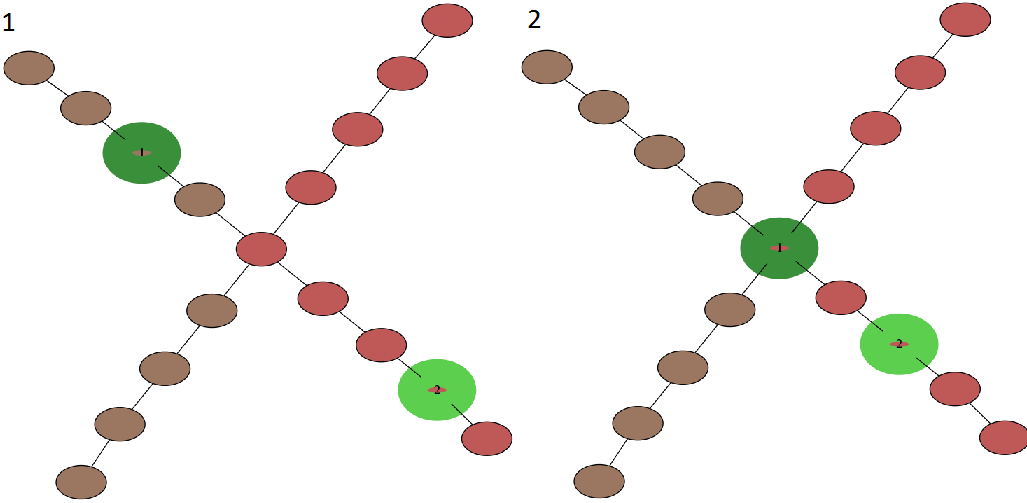
\includegraphics[width=1.0\textwidth]{collision-avoidance-crossroads.png}
  \caption{Unikanie kolizji na skrzyżowaniu}
  \label{collision-avoidance-crossroads}
\end{figure}
\newpage

\section{Format danych wejściowych}

Zaprezentowane rozwiązanie potrzebuje dane na temat skrzyżowań, samochodów oraz ograniczeń parametrów samochodów. Skrzyżowania reprezentowane są w pliku CSV \footnote{CSV - wartości rozdzielone przecinkiem. Format przechowywania danych w pliku tekstowym, gdzie pierwszy wiersz opisuje wartości. Następne wiersze to wartości atrybutów opisanych w wierszu pierwszym. } posiadającym atrybuty: numer drogi, rozmiar, przecięcia, kierunek. Przecięcie reprezentowane są przez dwie liczby. Na przykład 5 7 - oznacza, że droga przecina drogę o numerze 5 w pozycji 7. Kolejne przecięcia oddzielane są średnikami. Stany samochodów zapisane są w pliku CSV posiadającym atrybuty: numer samochodu, numer drogi samochodu, pozycję na drodze, pozycję końcową. Ograniczenia przechowywane są w osobnym pliku CSV posiadającym atrybuty: maksymalna prędkość, parametr bezpieczeńśtwa, wartości przyspieszeń.

\section{Funkcja heurystyki}

Funkcja heurystyki dla algorytmu A* jest to suma kroków czasowych, po których wszystkie auta przekroczą ostatnie skrzyżowanie - czyli osiągną cel. Funkcja liczona jest, przy założeniu, że wszystkie samochody maksymalnie przyspieszają.
\newline
\indent
W opracowanym rozwiązaniu każdy samochód ma wyznaczoną pozycję, na której musi się znaleźć lub ją przekroczyć (jest to pozycja za ostatnim skrzyżowaniem). Poniżej przedstawiony jest przykład liczonej funkcji heurystyki dla dwóch stanów opisujących położenia samochodów na skrzyżowaniu.
\newpage
\begin{table}[t]
    \begin{tabular}{|c|c|c|c|c|}
      \hline 
      Numer pojazdu & Numer drogi & Pozycja na drodze & Prędkość & Pozycja końcowa\\
      \hline
      1 & 1 & 1 & 1 & 6 \\
      \hline
      2 & 2 & 1 & 1 & 6 \\
      \hline
      3 & 3 & 1 & 1 & 6 \\
      \hline
      4 & 4 & 1 & 1 & 6 \\
      \hline
    \end{tabular} 
    \caption{Stan 1}
    \label{FirstState}
\end{table}
\begin{table}[t]
    \begin{tabular}{|c|c|c|c|c|}
      \hline 
      Numer pojazdu & Numer drogi & Pozycja na drodze & Prędkość & Pozycja końcowa\\
      \hline
      1 & 1 & 1 & 0 & 6 \\
      \hline
      2 & 2 & 1 & 1 & 6 \\
      \hline
      3 & 3 & 1 & 0 & 6 \\
      \hline
      4 & 4 & 1 & 1 & 6 \\
      \hline
    \end{tabular} 
    \caption{Stan 2}
    \label{SecondState}
\end{table}
\newpage
Dla stanu opisanego w tabeli \ref{FirstState} funkcja heurystyki jest liczona następująco:
\newline
\newline
\textbf{Dla pojazdów 1-4:}
\newline
\newline
\underline{1 krok czasowy}:
\newline
\newline
prędkość = (prędkość) 1 + (maksymalne przyspieszenie) 1 = 2
\newline
pozycja = (pozycja) 1 + (prędkość) 2 = 3
\newline
\newline
Pojazd znajduje się na pozycji 3, która jest przed pozycją końcową 6 - liczony jest kolejny krok czasowy.
\newline
\newline
\underline{2 krok czasowy}:
\newline
\newline
prędkość = (prędkość) 2 + (maksymalne przyspieszenie) 1 = 3
\newline
pozycja = (pozycja) 3 + (prędkość) 3 = 6
\newline
\newline
Pojazd znajduje się na pozycji 6, która jest równa pozycji końcowej.
\newline
\newline
Razem 2 kroki czasowe dla jednego pojazdu. Dla wszystkich czterech pojazdów - 8 kroków czasowych.
\newline
\newline
\newline
Dla stanu opisanego w tabeli \ref{SecondState} funkcja heurystyki jest liczona następująco:
\newline
\newline
\textbf{Dla pojazdów 1 i 3}
\newline
\newline
\underline{1 krok czasowy}:
\newline
\newline
prędkość = (prędkość) 0 + (maksymalne przyspieszenie) 1 = 1
\newline
pozycja = (pozycja) 1 + (prędkość) 1 = 2
\newline
\newline
Pojazd znajduje się na pozycji 2, która jest przed pozycją końcową 6 - liczony jest kolejny krok czasowy.
\newline
\newline
\underline{2 krok czasowy}:
\newline
\newline
prędkość = (prędkość) 1 + (maksymalne przyspieszenie) 1 = 2
\newline
pozycja = (pozycja) 2 + (prędkość) 2 = 4
\newline
\newline
Pojazd znajduje się na pozycji 4, która jest przed pozycją końcową 6 - liczony jest kolejny krok czasowy.
\newline
\newline
\underline{3 krok czasowy}:
\newline
\newline
prędkość = (prędkość) 2 + (maksymalne przyspieszenie) 1 = 3
\newline
pozycja = (pozycja) 4 + (prędkość) 3 = 7
\newline
\newline
Pojazd znajduje się na pozycji 7, która jest za pozycją końcową 6.
\newline
\newline
Razem 3 kroki czasowe dla jednego pojazdu. Dla pojazdów 1 i 3 - 6 kroków czasowych.
\newline
\newline
\textbf{Dla pojazdów 2 i 4:}
\newline
\newline
\underline{1 krok czasowy}:
\newline
\newline
prędkość = (prędkość) 1 + (maksymalne przyspieszenie) 1 = 2
\newline
pozycja = (pozycja) 1 + (prędkość) 2 = 3
\newline
\newline
Pojazd znajduje się na pozycji 3, która jest przed pozycją końcową 6 - liczony jest kolejny krok czasowy.
\newline
\newline
\underline{2 krok czasowy}:
\newline
\newline
prędkość = (prędkość) 2 + (maksymalne przyspieszenie) 1 = 3
\newline
pozycja = (pozycja) 3 + (prędkość) 3 = 6
\newline
\newline
Pojazd znajduje się na pozycji 6, która jest równa pozycji końcowej.
\newline
\newline
Razem 2 kroki czasowe dla jednego pojazdu. Dla pojazdów 2 i 4 - 4 kroki czasowe.
\newline
\newline
Razem dla wszystkich pojazdów - 10 kroków czasowych.
\newline
\newline
\newline
Podsumowując, dla stanu opisanego w tabeli \ref{FirstState} funkcja heurystyki zwróci wartość 8 (osiem kroków czasowych), a dla stanu opisanego w tabeli \ref{SecondState} funkcja heurystyki zwróci wartość 10 (dziesięć kroków czasowych). Algorytm w pierwszej kolejności wybierze wartość minimalną - czyli wybierze stan opisany w tabeli \ref{FirstState}.

\section{Złożoność rozwiązania}

W przedstawionym modelu stan jednego samochodu to (p, v), gdzie p to pozycyja na drodzę oraz v to prędkość pojazdu w odcinkach drogi na krok czasowy. Pozostałe parametry, czyli numer drogi na której znajduje się samochód i pozycja końcowa czy przyspieszenie nie zmieniają się. Dla wartości przyspieszeń ze zbioru \{-1, 0, 1\} dla samochodu powstają następujące stany:
\begin{enumerate}
\item (p + v, v) - dla przyspieszenia 0
\item (p + v + 1, v + 1) - dla przyspieszenia 1
\item (p + v - 1, v - 1) - dla przyspieszenia 1
\end{enumerate}
Dla jednego pojazdu z każdym krokiem czasowym powstają 3 stany. Mając na skrzyżowaniu 12 pojazdów otrzymujemy daje 531441 możliwości w jednym kroku czasowym. Algorytm nie musi przechodzić przez wszystie możliwości, jeżeli wcześniej znajdzie rozwiązanie.
\newline
\indent
Największym obciążeniem algorytmu jest unikanie kolizji. Zajmuje ono około 60 \% czasu znajdowania rozwiązania. Jest to spowodowane tym, że dla każdego stanu, którym jest położenie wszystkich pojazdów na skrzyżowaniu, algorytm przeprowadza dwie weryfikacje w każdym kroku czasowym:
\begin{enumerate}
\item Czy istnieją dwa pojazdy, które w tym samym czasie przekroczyły skrzyżowanie
\item Czy odcinki zajęte przez dwa pojazdy na jednym pasie się przecinają
\end{enumerate}
Powyższe stany eliminowane są z rozwiązania co zapewnia unikanie kolizji.
\newline
\indent
Dla zbioru przyspieszeń \{-2, -1, 0, 1, 2\} dla każdego pojazdu powstaje 5 stanów. Mając na skrzyżowaniu 12 pojazdów mamy 244140625 możliwości w jednym kroku czasowym. Możliwości przypadające na krok czasowy są silnie związane z czasem wykonania algorytmu. Wraz ze wzrostem liczby pojazdów na skrzyżowaniach, a co za tym idzie dodatkowych możliwości, czas wykonania rośnie ekspotencjalnie.
\section{Reprezentacja graficzna wyników}

W celu graficznej reprezentacji wyników zaimplementowany został moduł graficzny. Działanie modułu graficznego oparte jest na rysowaniu grafów z wykorzystaniem biblioteki Graphviz \footnote{Graphviz - to zestaw narzędzi do tworzenia diagramów za pomocą grafów. Jest rozwijany jako otwarte oprogramowanie i udostępniany na licencji CPL} oraz jej implementacji w języku Ruby. Skrzyżowanie jest reprezentowane za pomocą grafu. Wierzchołkami grafu są poszczególne odcinki dróg. Krawędziami grafu są połączenia pomiędzy odcinkami. Samochody poruszające się po tej samej drodze są zaznaczone grubszym obwodem oraz mają ten sam kolor. Samochody można rozróżnić poprzez unikatowy numer na nich napisany. Kolejne kroki czasowe reprezentowane są poprzez następne grafy z kolejnymi ułożeniami samochodów. Efektem końcowym jest stworzony GIF z następujących po sobie grafów przy użyciu biblioteki 'rmagick' dla języka Ruby.
\newline
\indent
Moduł graficzny wczytuje wszystkie dane wejściowe: pozycję samochodów, dane skrzyżowania oraz ograniczenia. Kolejno na wejście otrzymuje plik zawierający JSON \footnote{JSON - lekki format tekstowy wymiany danych komputerowych}, który reprezentuje wszystkie stany samochodów na skrzyżowaniach od momentu startu, aż do opuszczenia skrzyżowań przez wszystkie samochody. Plik powstaje w wyniku wykonania zaprezentowanego algorytmu A*. Moduł wczytując dane początkowe tworzy graf bazowy. Graf bazowy przedstawia skrzyżowanie wraz z pojazdami. Kolory dla dróg oraz samochodów są losowane oraz przetrzymywane w zbiorze tak, aby żaden z kolorów się nie powtórzył. Następnie moduł, posiadający kolejne stany w kolejnych krokach czasowych, korzysta z grafu bazowego i zmienia pozycję samochodów. Po każdym kroku czasowym zapisywane jest zdjęcie grafu z numerem kroku czasowego.
\newline
\indent
W module znajduje się także dodatkowe sprawdzanie kolizji. Jeżeli kolizja wystąpi, w danym kroku czasowym na zdjęciu dodany zostanie napis "Collision". Dzięki temu można zobaczyć prawdopodobieństwo kolizji w przypadku, gdy jeden z pojazdów nie zastosuje się do planu.
\newline
\indent
Na rysunku \ref{graphical-framework} zaprezentowane jest działanie modułu graficznego dla skrzyżowania czterech dróg i ośmiu pojazdów. Na 11 elemencie rysunku widać, że wszystkie samochody opuściły wszystkie skrzyżowania po 11 krokach czasowych.
\begin{figure}[H]
    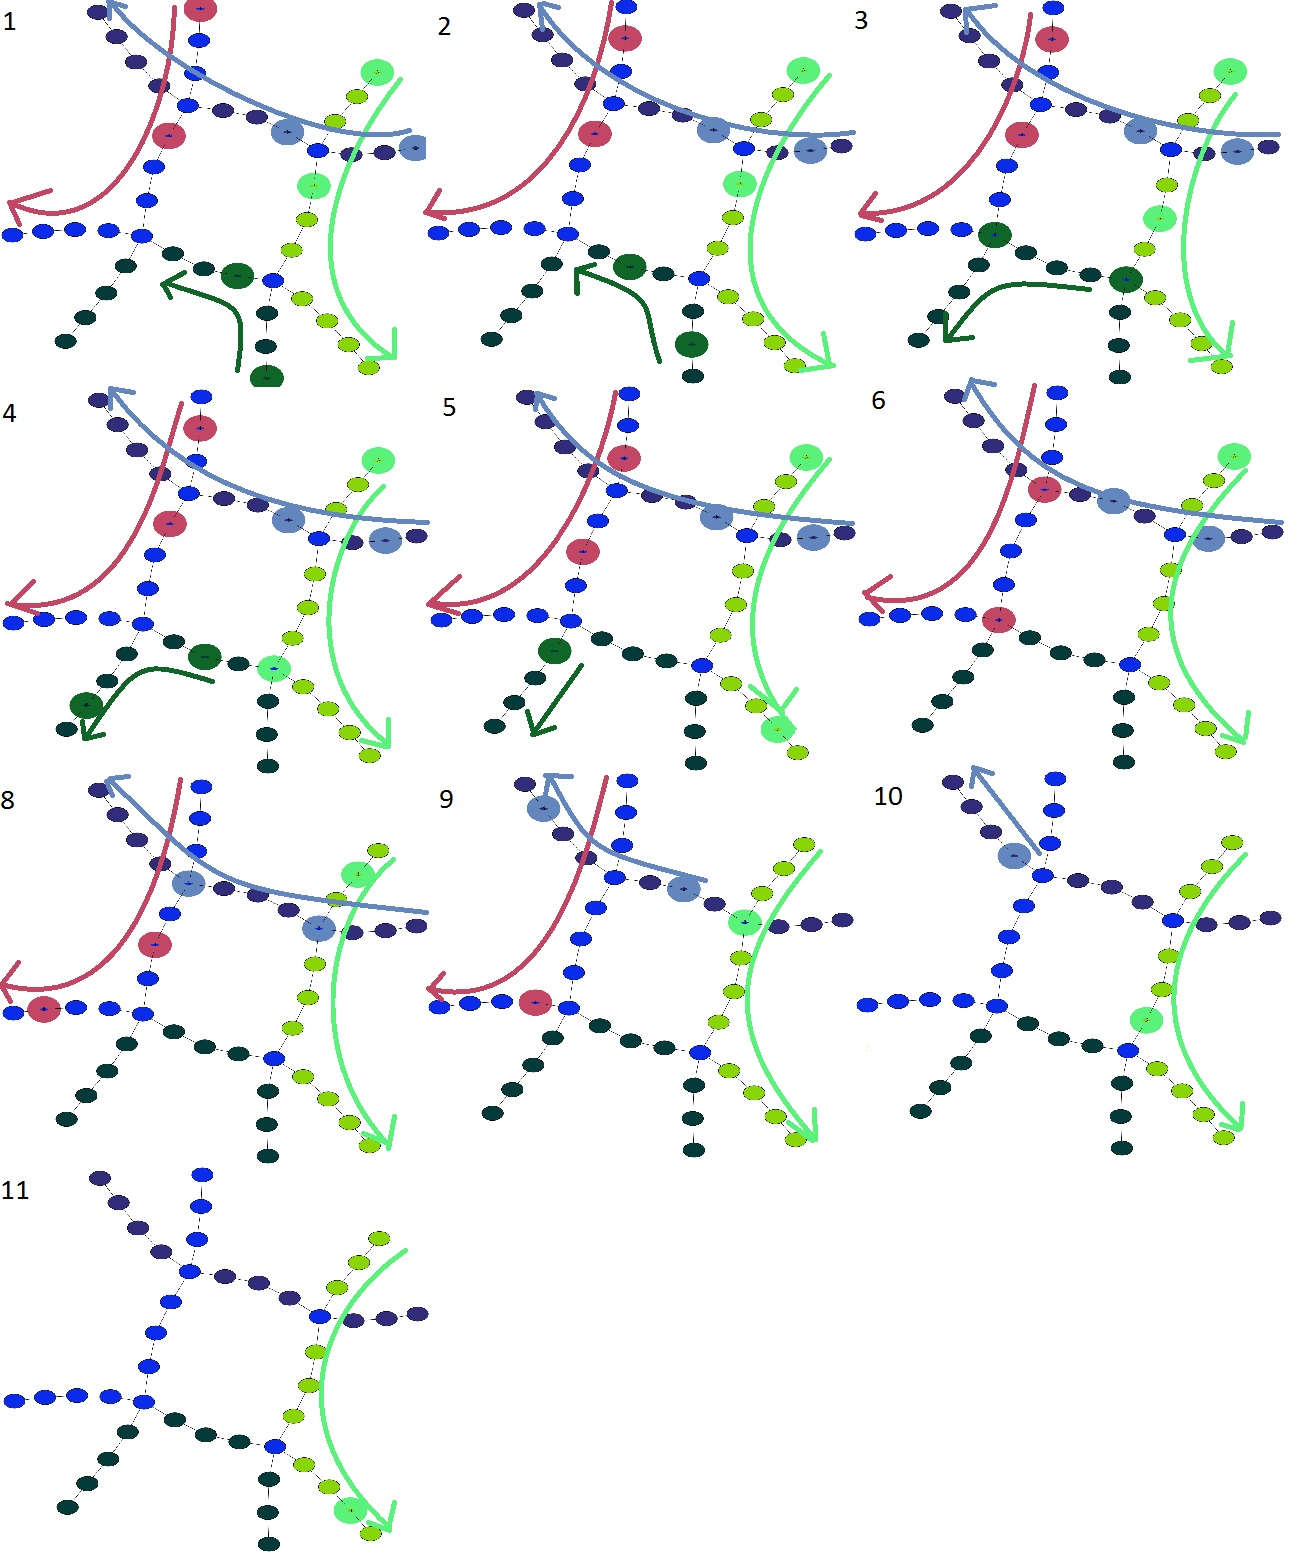
\includegraphics[width=1.0\textwidth]{graphical_module_2.png}
  \caption{Wynik działania modułu graficznego}
  \label{graphical-framework}
\end{figure}
\newpage

\mychapter{5}{5. Wyniki} \label{chap:outcomes}

\section{Wstęp}

W~celu zbadania działania systemu przeprowadzone zostały następujące pomiary:
\begin{itemize}
\item Pomiar czasu wykonania programu w~zależności od liczby samochodów na skrzyżowaniu 
\item Pomiar ilości kroków czasowych, po których wszystkie samochody opuszczą skrzyżowania w~zależności od liczby samochodów na skrzyżowaniu
\end{itemize}

Pomiary zostały wykonane na dwóch sieciach dróg:
\begin{itemize}
\item Skrzyżowanie ze sobą ośmiu dróg
\item Skrzyżowanie ze sobą czterech dróg
\end{itemize}

Drogi na obydwu sieciach mają rozmiar 24. Reprezentacja graficzna skrzyżowań jest przedstawiona na rysunku \ref{both-crossroads} z~przykładowymi rozmieszczeniami pojazdów.
\begin{figure}[H]
    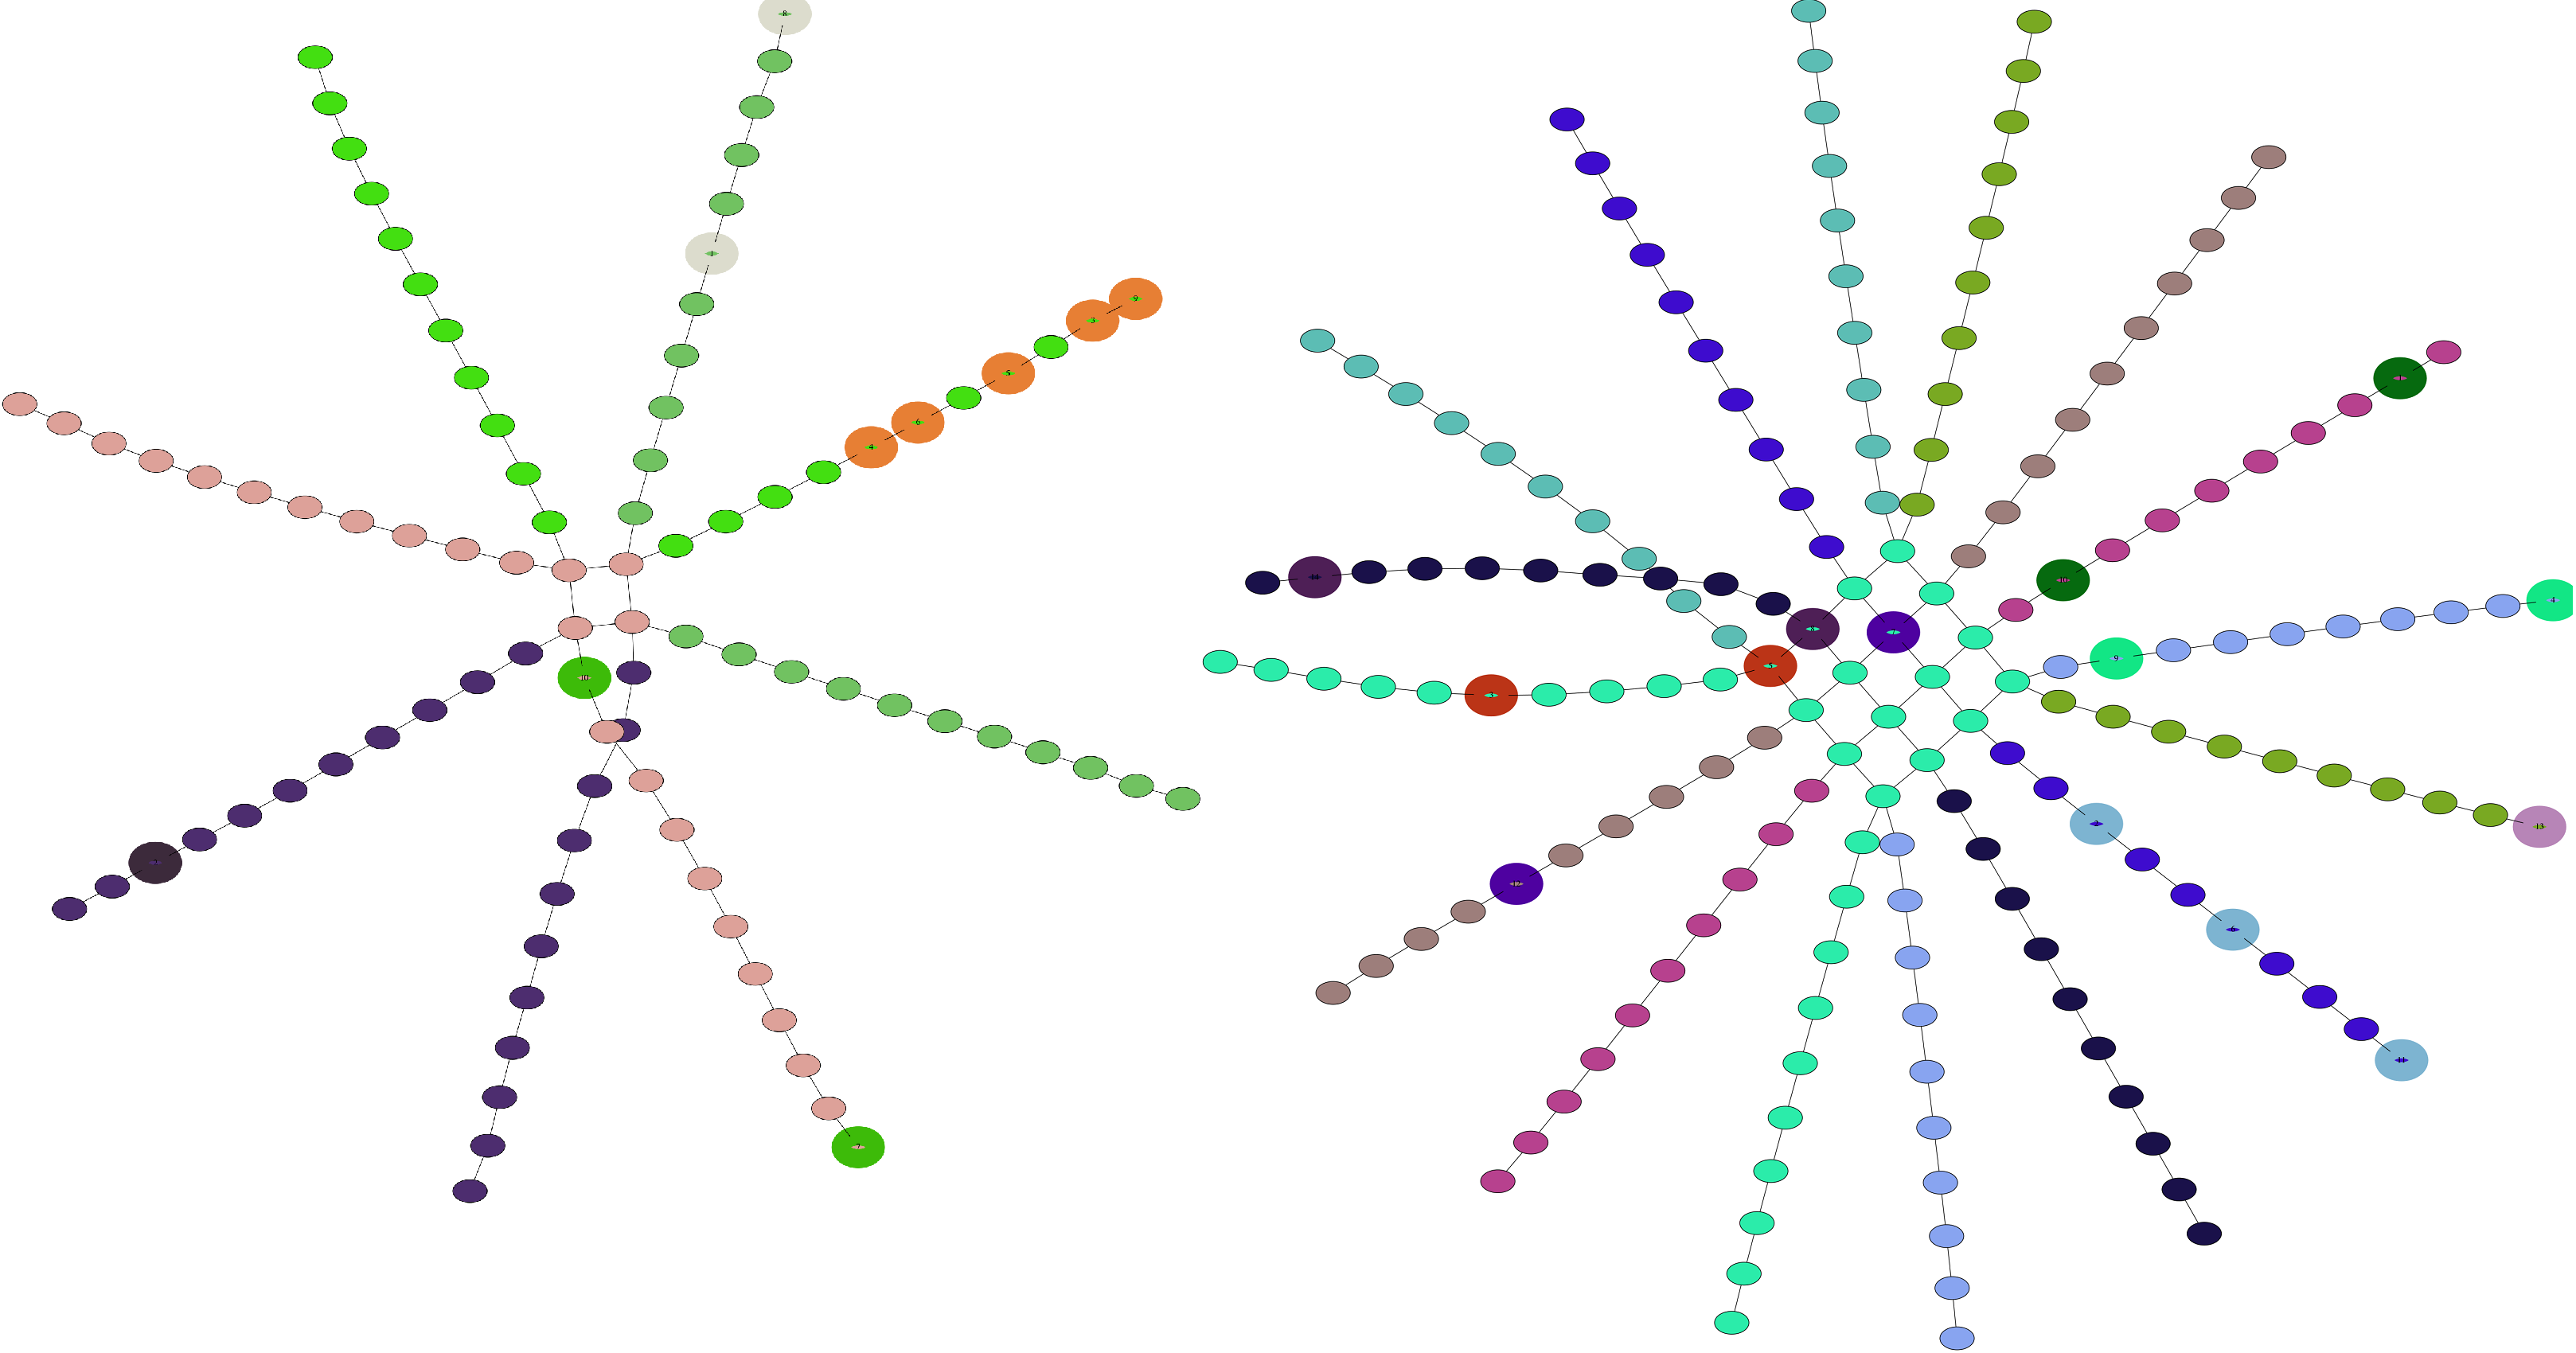
\includegraphics[width=1.0\textwidth]{2_crossroads.png}
  \caption{Skrzyżowanie czterech oraz ośmiu dróg}
  \label{both-crossroads}
\end{figure}

Pomiary zostały przeprowadzone dla następującej liczby samochodów \{2, 4, 6, 8, 10, 12\}. Dla każdej liczby samochodów wygenerowane losowo zostało 30 położeń pojazdów przy założeniu, że żaden z~pojazdów nie startuje za ostatnim skrzyżowaniem. Skrypt losujący przyjmuje jako dane wejściowe opis sieci skrzyżowań, liczbę samochodów oraz liczbę stanów startowych do wygenerowania.
\newline
\newline
Pomiary zostały wykonane na następującym sprzęcie:
\begin{itemize}
\item Procesor: Intel(R) Core(TM) i7-4700MQ CPU @ 2.40GHz
\item Liczba rdzeni procesora: 2 - Obliczenia zostały wykonane na jednym wątku
\item 16 GB pamięci RAM
\end{itemize}

\section{Wyniki pomiarów dla skrzyżowania czterech dróg}

Zgodnie z~wcześniej opisanymi założeniami dla skrzyżowania czterech dróg, program został uruchomiony 30 razy dla samochodów ze zbioru \{2, 4, 6, 8, 10, 12\} co razem daje 180 uruchomień.
\newline
\newline
Wykresy przedstawiające wyniki na skrzyżowaniu czterech dróg zaprezentowane są na rysunku \ref{4_roads_execution_time_new} oraz \ref{four-roads-crossroads-timesteps}
\begin{figure}[H]
  \centering
  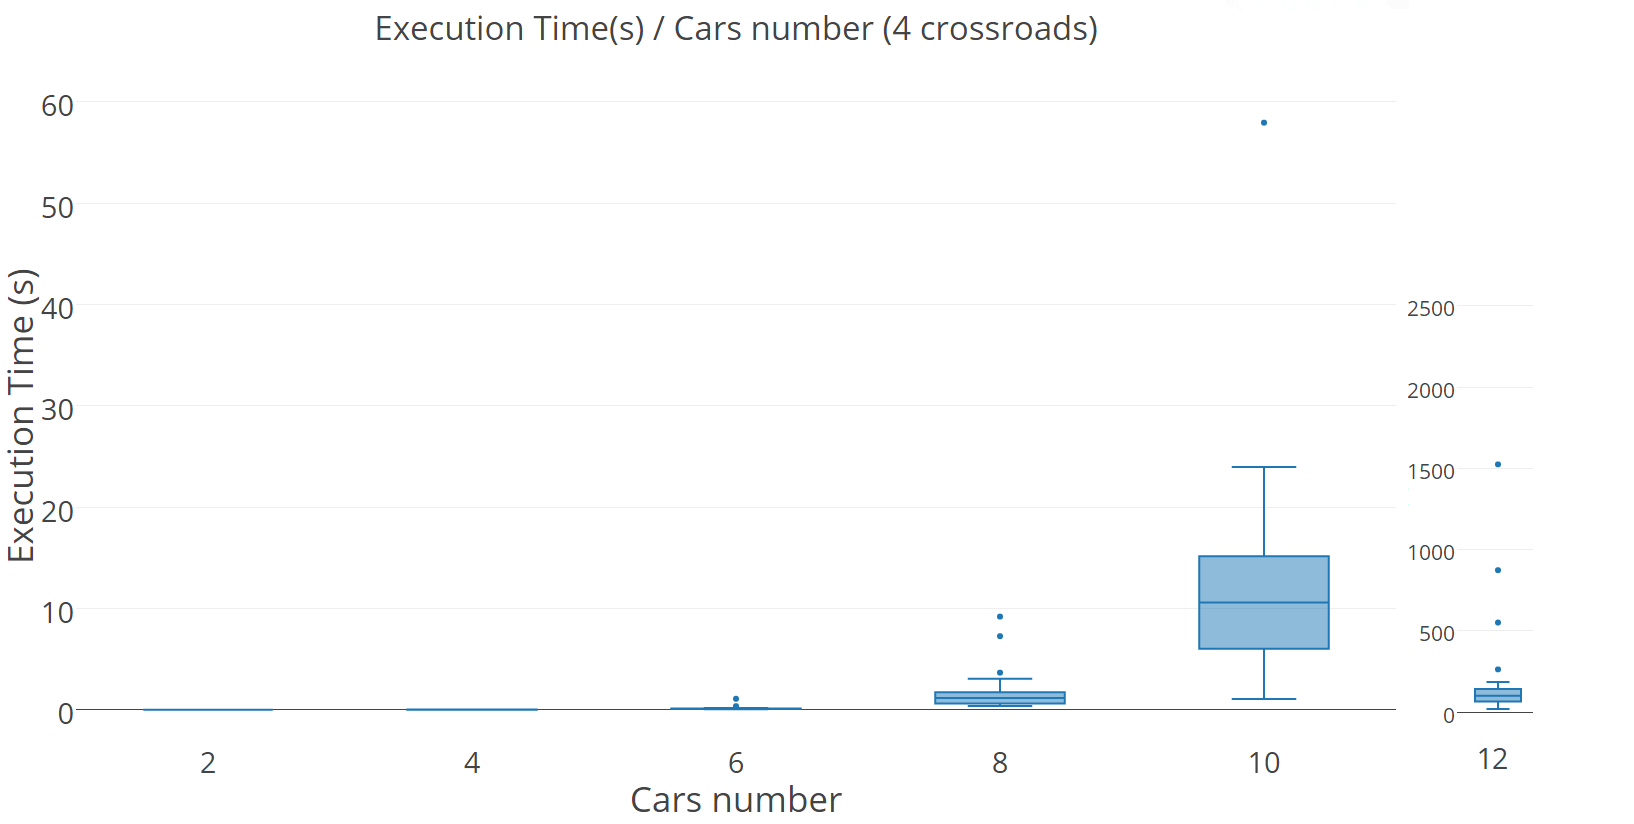
\includegraphics[width=1.0\textwidth]{4_roads_execution_time_new.png}
  \caption{Wykres zależności czasu wykonania programu od liczby pojazdów}
  \label{4_roads_execution_time_new}
\end{figure}
\begin{figure}[H]
  \centering
  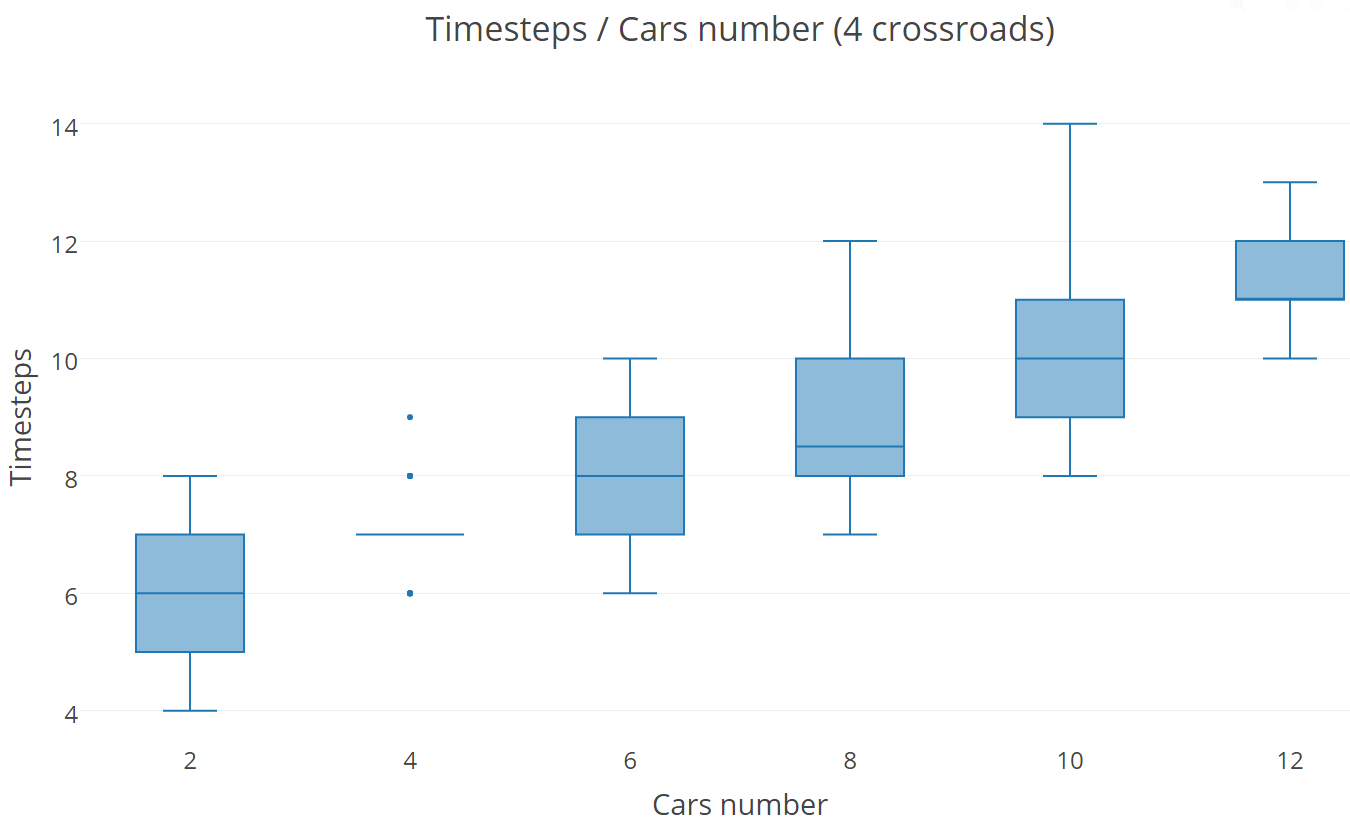
\includegraphics[width=1.0\textwidth]{4_roads_timesteps_new.png}
  \caption{Wykres zależności kroków czasowych od liczby pojazdów}
  \label{four-roads-crossroads-timesteps}
\end{figure}

\section{Wyniki pomiarów dla skrzyżowania ośmiu dróg}

Dla skrzyżowania ośmiu dróg też zostało przeprowadzone 180 uruchomień. Wykresy przedstawiające wyniki na skrzyżowaniu ośmiu dróg zaprezentowane są na rysunkach \ref{8_roads_execution_time_new} oraz \ref{8_roads_timesteps_new}
\begin{figure}[H]
  \centering
  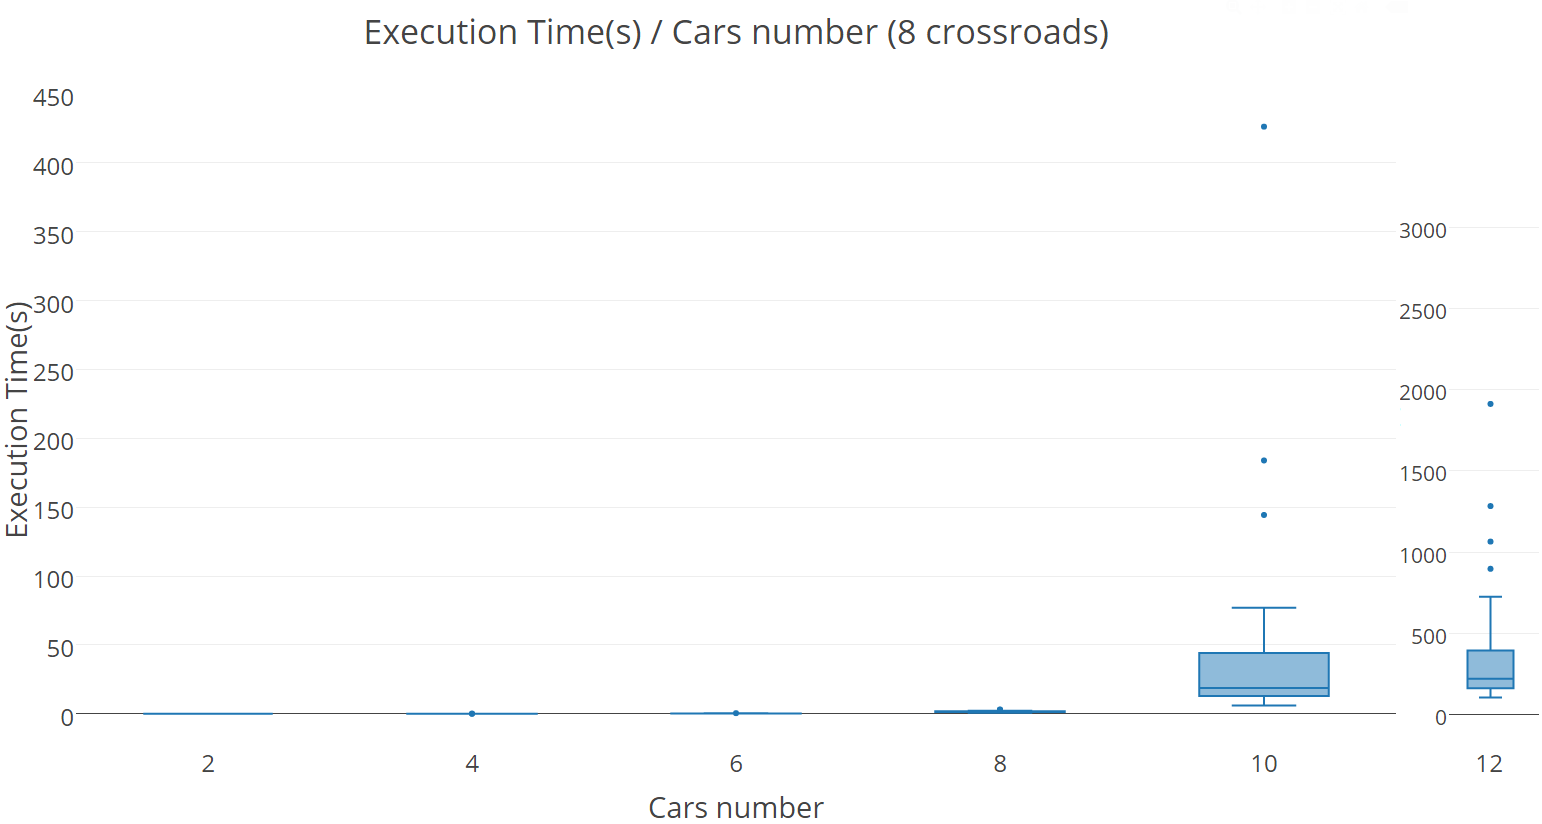
\includegraphics[width=1.0\textwidth]{8_roads_execution_time_new.png}
  \caption{Wykres zależności czasu wykonania programu od liczby pojazdów}
  \label{8_roads_execution_time_new}
\end{figure}
\begin{figure}[H]
  \centering
  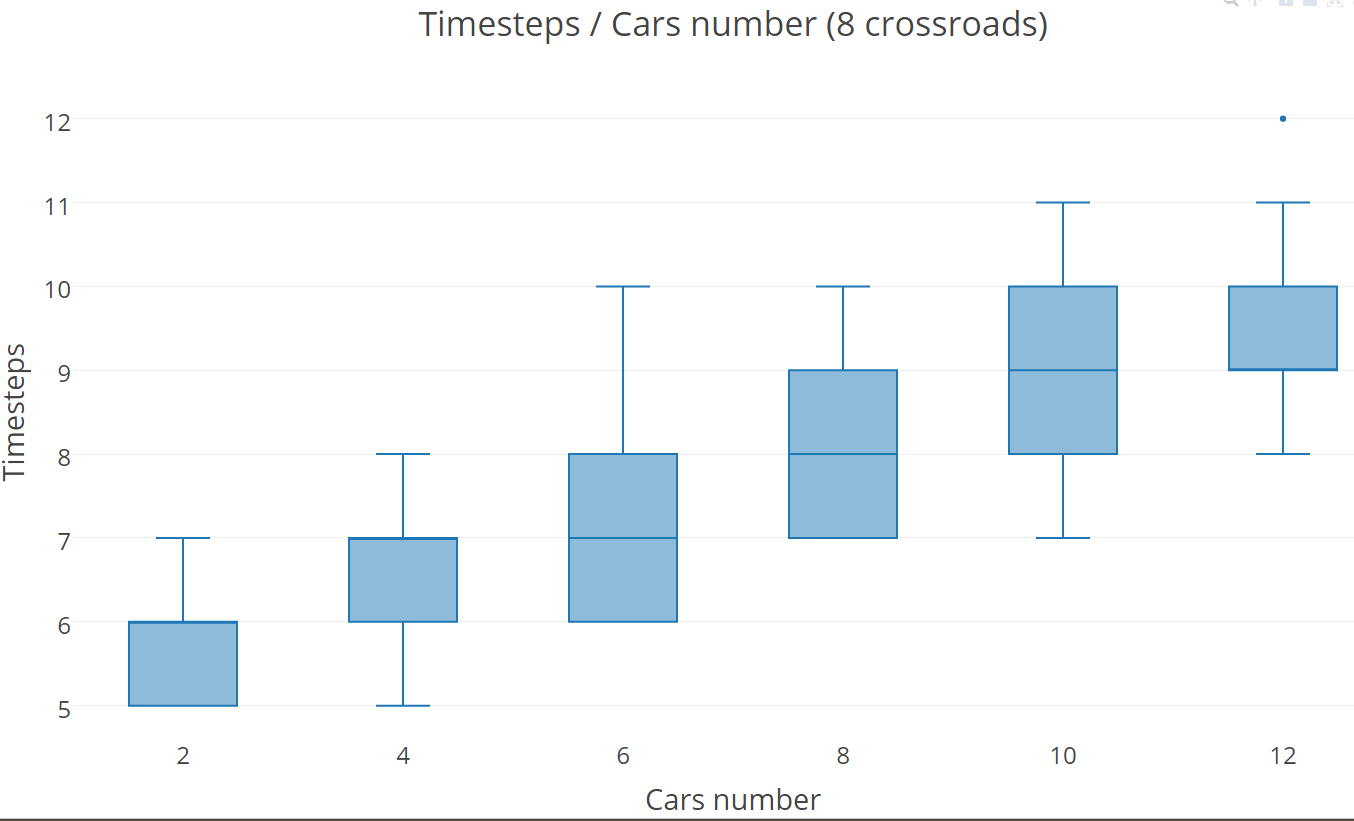
\includegraphics[width=1.0\textwidth]{8_roads_timesteps_new.png}
  \caption{Wykres zależności kroków czasowych od liczby pojazdów}
  \label{8_roads_timesteps_new}
\end{figure}

\section{Wnioski z~pomiarów na skrzyżowaniach czterech i~ośmiu dróg}

Wykresy zależności czasu wykonywania względem liczby samochodów na skrzyżowaniu pokazują ograniczenie metody względem liczby samochodów. Jak widać, czas wykonania rośnie ekspotencjalnie względem liczby samochodów. Dla 12 pojazdów czas wykonania przekracza nawet 25 minut. Dla sieci skrzyżowań, na której jest 12 lub więcej samochodów użycie metody jest zbyt czasochłonne.
\newline
\indent
Wykresy zależności liczby kroków czasowych, po których wszystkie samochody opuszczą skrzyżowania pokazują, że liczba kroków czasowych rośnie liniowo względem liczby pojazdów. 
\newline
\indent
Liczba kroków czasowych na skrzyżowaniu ośmiu dróg jest mniejsza niż na skrzyżowaniu czterech dróg. Spowodowane jest to tym, że na skrzyżowaniu czterech dróg auta stoją jedno za drugim na pasach, bez wolnej przestrzeni przed sobą. W~porównaniu do skrzyżowania ośmiu dróg auta mogą swobodnie poruszać się na pasie i~częściej wymijają kolizję na skrzyżowaniu.

\section{Prawdopodobieństwo kolizji}

W~celu przetestowania bezpieczeństwa rozwiązania zostały przeprowadzone pomiary prawdopodobieństwa kolizji w~przypadku pomyłek pojazdów. Pomyłka polega na niezastosowaniu się pojazdu do planu. W~rozwiązaniu zaimplementowane zostało symulowanie kolizji pojazdów z~określonym prawdopodobieństwem. W~każdym kroku czasowym każdy z~pojazdów myli się z~podanym wcześniej prawdopodobieństwem. Wynikiem pomiarów jest zależność prawdopodobieństwa kolizji od prawdopodobieństwa pomyłki. Zmierzone zostało prawdopodobieństwo kolizji w~razie pomyłek pojazdów z~następującymi prawdopodobieństwami \{0.001, 0.005, 0.01\}
\newline
\indent
W~obliczeniach pod uwagę wzięty został także parametr bezpieczeństwa. Pomiary zostały wykonane dla skrzyżowania 8 dróg, na których znajdowało się 10 pojazdów. Program uruchomiony został 30 razy dla parametru bezpieczeństwa równego 0 oraz 30 razy dla parametru bezpieczeństwa równego 1, aby pokazać, jakie bezpieczeństwo gwarantuje użycie tego parametru.
\newline
\newline
Wyniki z~parametrem bezpieczeństwa równym 0 zaprezentowane są w~tabeli \ref{firstCollision}
\begin{table}[H]
    \centering
    \begin{tabular}{|c|c|c|c|}
      \hline 
      Prawdopodobieństwo pomyłki & 0.001 & 0.005 & 0.01 \\
      \hline
      Prawdopodobieństwo kolizji & 0.2 & 0.27 & 0.54 \\
      \hline
    \end{tabular} 
    \caption{Prawdopodobieństwo kolizji z~parametrem bezpieczeństwa równym 0}
    \label{firstCollision}
\end{table}
\noindent
Wyniki z~parametrem bezpieczeństwa równym 1 zaprezentowane są w~tabeli \ref{secondCollision}
\begin{table}[H]
    \centering
    \begin{tabular}{|c|c|c|c|}
      \hline 
      Prawdopodobieństwo pomyłki & 0.001 & 0.005 & 0.01 \\
      \hline
      Prawdopodobieństwo kolizji & 0 & 0 & 0.24 \\
      \hline
    \end{tabular} 
    \caption{Prawdopodobieństwo kolizji z~parametrem bezpieczeństwa równym 0}
    \label{secondCollision}
\end{table}
Jak pokazują wyniki w~tabelach \ref{firstCollision}, \ref{secondCollision} parametr bezpieczeństwa niweluje prawdopodobieństwo kolizji dla małych prawdopodobieństw (0.001, 0.005) pomyłki do zera. Dla prawdopodobieństwa pomyłki równego 0.01 parametr bezpieczeństwa nie zapobiega całkowicie kolizjom - w~przeprowadzonych badaniach zmniejszył je o~30\%.

\section{Porównanie wyników z~rozwiązaniem ze światłami drogowymi}

W~celu zweryfikowania szybkości podejścia z~wykorzystaniem algorytmu A* wyniki zostały porównane z~rozwiązaniem polegającym na optymalizacji świateł drogowych przedstawionym w~pracy \cite{slakomy}. Porównywane rozwiązanie także jest oparte o~kroki czasowe. Drogi także są dyskretne, mierzone w~odcinkach, a~prędkość też mierzona jest w~ilości odcinków drogi na krok czasowy.
\newline
\indent
Rozwiązania różnią się modelami danych, które reprezentują skrzyżowania oraz znajdujące się na nich pojazdy. W~jednym rozwiązaniu położenie i~droga aut jest określona za pomocą grafu oraz wierzchołków grafu, przez które auta będą przechodzić. W~opisywanym w~tej pracy, rozwiązaniu drogi są opisywane poprzez ich rozmiar oraz przecięcia z~innymi drogami. Położenia samochodów natomiast poprzez numer drogi oraz numer odcinka drogi, na której się znajdują.
\newline
\indent
Wykonując pomiary, uzgodnione zostały wspólne warunki w~obu rozwiązaniach tak, aby można było je porównać. Porównywane są kroki czasowe, po których wszystkie auta opuszczą skrzyżowanie. Wspólne warunki są następujące:
\begin{itemize}
\item Maksymalna prędkość samochodów wynosi 4 odcinki drogi na krok czasowy
\item Wartości przyspieszeń pojazdów są następujące: \{-1, 0, 1\}
\item Losowane położenia pojazdów w~celu wykonania 30 pomiarów są wykonywane w~taki sposób, aby żaden pojazd nie znajdował się za skrzyżowaniem
\item Rozwiązanie kończy obliczenia, kiedy wszystkie pojazdy znajdą się za skrzyżowaniem
\item Pomiary zostały wykonane na skrzyżowaniu ośmiu dróg dla następujących liczb pojazdów \{2, 4, 6, 8, 10 ,12\}
\item Drogi mają rozmiar 24
\end{itemize}
Wykres z~wynikami pokazany jest na rysunku \ref{comparison}
\begin{figure}[H]
  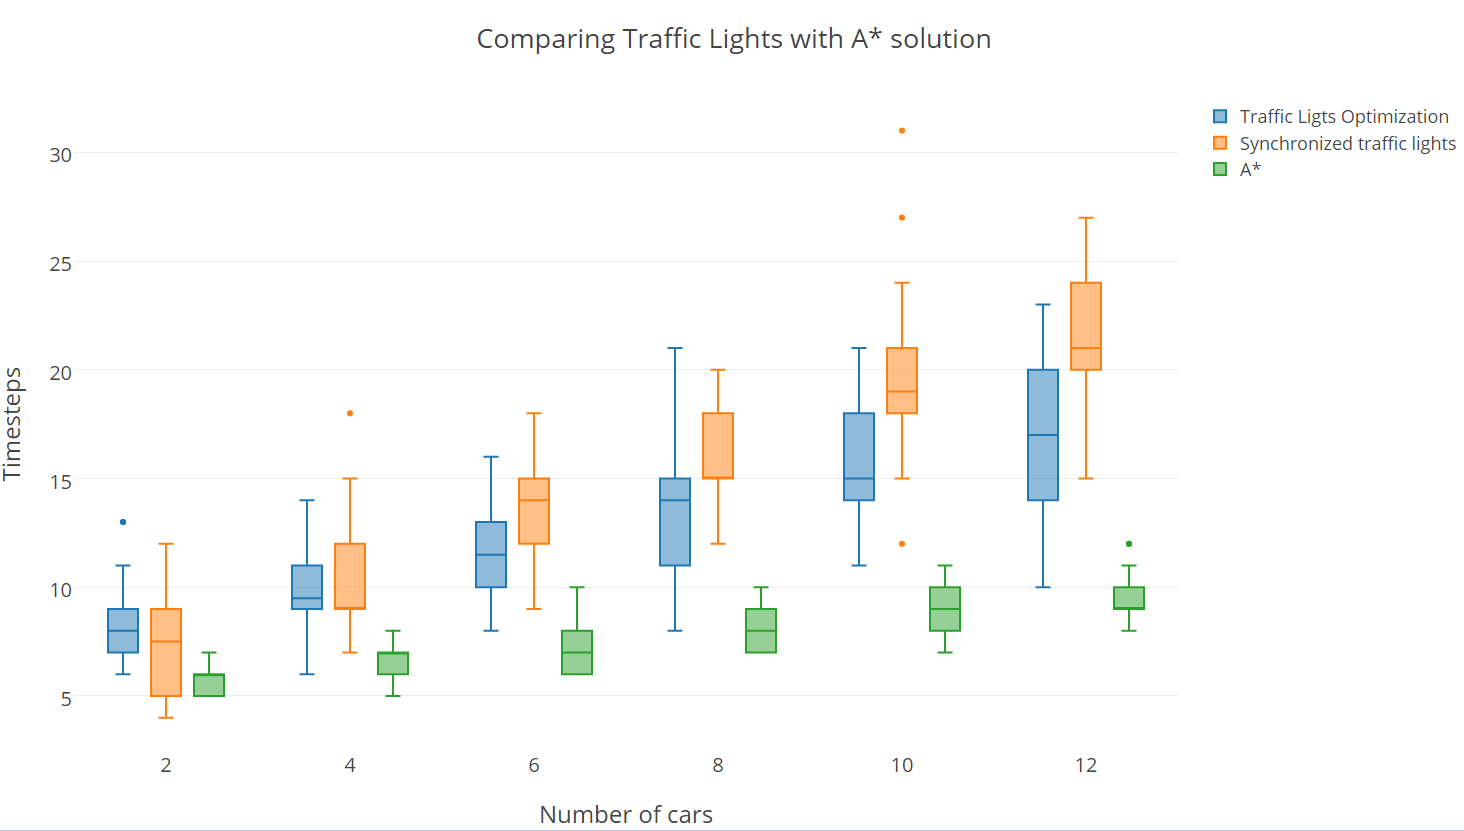
\includegraphics[width=1.0\textwidth]{8_roads_comparison_2.png}
  \caption{Porównanie rozwiązania z~użyciem A* ze światłami drogowymi na skrzyżowaniu ośmiu dróg}
  \label{comparison}
\end{figure}
Rozwiązanie z~wykorzystaniem algorytmu A* daje lepsze wyniki na tle rozwiązania ze światłami sekwencyjnymi oraz z~ich optymalizacjami. Zgodnie z~przedstawioną tezą, przepustowość na skrzyżowaniach jest lepsza w~rozwiązaniu A* w~porównaniu do świateł. Rozwiązanie korzystające z~algorytmu A* dla 12 pojazdów nie przekracza 15 kroków czasowych. Dla świateł zoptymalizowanych przekracza 20 kroków czasowych, a~dla świateł sekwencyjnych przekracza 25 kroków czasowych. Przedstawione w~pracy rozwiązanie zaoszczędza 5-10 kroków na jednym skrzyżowaniu dla 12 pojazdów. Wykorzystując metodę dla dużej sieci skrzyżowań, można zaoszczędzić dużo czasu.

\mychapter{6}{6. Zakończenie} \label{chap:conclusions}

\section {Podsumowanie}

W pracy przedstawiona została metoda planowania ruchu drogowego z wykorzystaniem algorytmu A*. Algorytm A* został zmodyfikowany - jest on generyczny, operuje na stanach oraz dynamicznie je przeszukuje. Implementacja algorytmu nie przeszukuje także całej przestrzeni stanów - algorytm kończy działanie w przypadku znalezienia pierwszego rozwiązania.
\newline
\indent
Analizując wyniki przedstawione w rozdziale 5 można wnioskować, że teza przedstawiona w rozdziale 3 jest prawdziwa. Porównanie opisywanej w tej pracy metody, wraz z koordynacją ruchu przy użyciu świateł drogowych pokazuje, że metoda daje lepsze wyniki, jeżeli chodzi o przepustowość. W przedstawionej metodzie, zapewnione jest także rozwiązywanie kolizji oraz bezpieczeństwo w przypadku niezastosowania się pojazdów do planu. Rozwiązanie zostało zaprojektowane i uruchamiane na jednym wątku procesora. Używając więcej wątków, można liczyć plany wielowariantowe w celu szybkiej reakcji na pomyłki pojazdów.
\newline
\indent
Jak pokazują wyniki, zastosowanie metody do koordynacji ruchu na skrzyżowaniu ze sobą ośmiu dróg zaoszczędza 20-40\% kroków czasowych. Korzystając z metody dla większej ilości sieci skrzyżowań, można zaoszczędzić dużo czasu.
\newline
\indent
Z pewnością wadą metody jest złożoność obliczeniowa, która rośnie ekspotencjalnie względem liczby pojazdów znajdujących się na sieci skrzyżowań. Obliczenia na opisanym w rozdziale 5 sprzęcie dla 14 pojazdów trwały nawet do kilku godzin.

\section{Kierunki rozwoju}

Metoda została zaprojektowana i uruchamiana na jednym wątku procesora. Głównym kierunkiem rozwoju jest liczenie planów wielowariantowych na wielu wątkach procesora. Mając równolegle wyliczane plany wielowariantowe, można następnie symulować pomyłki pojazdów, które polegają na niezastosowaniu się do planu głównego. Następnie, w przypadku takiej pomyłki pojazdu wykrywać ją i wysyłać pojazdom poprawiony plan ruchu. Mając wprowadzone takie zmiany, można kolejno policzyć prawdopodobieństwa kolizji w zależności od prawdopodobieństwa pomyłki pojedynczego pojazdu oraz minimalizować prawdopodobieństwo kolizji poprzez modyfikację parametru bezpieczeństwa.


\cleardoublepage % to ensure that the page reference is correct
\addcontentsline{toc}{chapter}{\listfigurename}
\listoffigures

\nocite{*} % forces bibtex to include all citations, whether or not they were referred to in the paper

\cleardoublepage
\addcontentsline{toc}{chapter}{Bibliography}
\bibliographystyle{bib-style}
\bibliography{bibliography}

\end{document}
